\section{Tactics}

A \newterm{tactic} is a scheme of equalities that can be used for rewriting.
When applied to a program term, any occurrence of the left-hand side is replaced by the right-hand side.
A valid application of a tactic is an instance of the scheme that is well-typed and logically valid
(that is, the two sides have the same interpretation in any structure that interprets the free
variables occurring in the equality).

The application of tactics yields a sequence of program terms, each of which is checked to
be equivalent to the previous one. We refer to this sequence by the name \newterm{development}.

We associate with each tactic some \newterm{proof obligations}, listed after the word {\bf Obligations}
in each of the following subsections.
When applying a tactic instance,
these obligations are also instantiated and given to an automated prover. If verified successfully,
they entail the validity of the instance. Clearly the tactic itself can be used as its proof obligation,
if it is easy enough to prove automatically; in such cases we write ``{\bf Obligations:} tactic.''

\newcommand\Obligations{\medskip\noindent{\bf Obligations:} }
\newcommand\reduce{\operatorname{reduce}}
\newcommand\listConcat{{\scriptstyle \,++\,}}

\subsection{Main Tactics}

\subsubsection{Slice}
\[f ~=~ f\big|_{X_1} ~\Big/~ f\big|_{X_2} ~\Big/ ~\cdots~ \Big/~ f\big|_{X_r}\]

This tactic partitions a mapping into sub-regions. Each $X_i$ may be a $\times$-expression
according to the arity of $f$.

\Obligations tactic.

Informally, the recombination expression is equal to $f$
when $X_{1..r}$ ``cover'' all the defined points of $f$ (also known as the \newterm{support} of $f$).

\subsubsection{Shrink}
\[f ~=~ f :: \T\]

Used to extra-specify the type of a sub-term.

\Obligations tactic.

For arrow-typed terms, this essentially requires to prove that $f$ is undefined anyway for
argument values outside the domain of $\T$, and that the defined values are in the range of $\T$.

\subsubsection{Stratify}
\[\fix (f\applt g) ~=~ \fix f ~\applt~ \psi\mapsto \fix (\dot\psi\applt g)\]
%
where $\dot\psi$ abbreviates $\theta\mapsto\psi$, with fresh variable $\theta$.

$\psi$ may be fresh, or it may reuse a variable already occurring in $g$, rebinding those occurrences.
The example of this section will illustrate why this is useful.

\Obligations Let $h=f\applt g$ and $g'=\psi\mapsto\dot\psi\applt g$. Let $\theta,\zeta$ be
fresh variables.
\begin{equation}
\renewcommand\arraystretch{1.5}
\begin{array}{l}
f\,(g'\,\zeta\,\theta) ~=~ f\,\zeta \\
g'\,(f\,\theta)\,\theta ~=~ h\,\theta
\end{array}
\label{tactics:Stratify obligations}
\end{equation}

Although the proof is not hard, we defer it to a later theorem.

\subsubsection{Synth}
\[\fix\big(h_1 ~\big/~ \cdots ~\big/~ h_r\big) ~=~ 
  (\fix f_1) :: \T_1 ~\big/~ \cdots ~\big/~ (\fix f_r) :: \T_r\]

This tactic is used to generate recursive calls to sub-programs. For $i=1..r$, $f_i$
is typically either $h_i$ or a sub-term occurring earlier in the development.

\Obligations Let $h=h_1/\cdots/h_r$, let $\overline\theta\!=\!\theta_{1..r}$ be $r$ fresh variables, and let
$f = \theta_{1..r} \mapsto (f_1\,\theta_1)::\T_1/\cdots/(f_r\,\theta_r)::\T_r$.
\begin{itemize}
  \item $\T_{1..r}$ are disjoint mappings.
  \item $h\,(f\,\overline\theta) = f\,\overline\theta$.
\end{itemize}

\subsection{Minor Tactics}

\subsubsection{Associativity}
\[\reduce\big\langle \reduce\langle\overline x\rangle, \reduce\langle\overline y\rangle\big\rangle ~=~ \reduce \langle \overline x, \overline y\rangle\]
%
where $\reduce$ is a built-in aggregation ($\min$, $\max$, $\Sigma$), 
and $x$, $y$ are lists of terms (of the same type).

\Obligations none.

\subsubsection{Distributivity}
Let $e$ be an expression with a hole, $e[\square] = (\cdots \square \cdots)$.
%
\[\renewcommand\arraystretch{1.2}
  \begin{array}{@{}r@{~}c@{~}l@{}}
    e[t_1/\cdots/t_r] &=& e[t_1] / \cdots / e[t_r] \\
    e[t_1/\cdots/t_r] &=& \reduce\langle e[t_1],\cdots,e[t_r]\rangle \\
    \reduce e[t_1/\cdots/t_r] &=& \reduce\langle \reduce e[t_1],\cdots,\reduce e[t_r]\rangle
  \end{array}\]

This tactic provides several alternatives for different uses of aggregations.
Clearly, $\big/$ does not distribute over any expression; we give just a few examples
where this tactic is applicable.
\begin{itemize}
  \item $(x/y)+1 ~=~ (x+1)~/~(y+1)$
  \item $x/0 ~=~ \max\langle x,0\rangle$ ~(for $x:\N$)
  \item $\min \big(f\big|_{J_0}~\big/~f\big|_{J_1}\big) ~=~
         \min\left\langle \min f\big|_{J_0} ~,~ \min f\big|_{J_1}\right\rangle$
\end{itemize}

\Obligations tactic.

\subsubsection{Elimination}
\[e[t] ~=~ e[\bot]\]
%
Used to eliminate a sub-term that is either always undefined or has no effect
in the context in which it occurs.

\Obligations tactic.

\subsubsection{Let Insertion}

Let $e$ be an expression with a hole, $e[\square] = (\cdots x_1 \mapsto \cdots x_k\mapsto \cdots \square \cdots)$, 
where $x_{1..k}\mapsto$ are abstraction terms enclosing $\square$. The bodies may contain arbitrary terms
in addition to these abstractions.
%
\[e[t] ~=~ (\overline{x}\mapsto t) ~\applt~ z\mapsto e[z\,\overline{x}]\]
%
where $\overline{x}=x_{1..k}$, and $z$ is either an existing or a fresh variable.

\Obligations tactic, if $z$ occurs free in $e$; otherwise none.

\subsubsection{Padding}
\[t ~=~ \big(t~/~f_1/\cdots/f_r\big) :: \T\]
%
where $\T$ is the type of $t$. This tactic is commonly used with Let insertion,
to make the type of a sub-term match the type of the entire term.

\Obligations tactic.


\subsection{Example \hrulefill}

For simplicity of the example, we assume that the input to the Simplified Gap problem
satisfies triangle inequalities:
%
\begin{equation}
w_{ij} \leq w_{ik} + w_{kj} \qquad w'_{ij} \leq w'_{ik} + w'_{kj}
\label{equ:triangle}
\end{equation}
%
for all (appropriately typed) $i<k<j$.

\medskip
Starting from the specification in \eqref{lang:gap spec}, we apply Synth to turn
$\fix (\theta\,i\,j\mapsto\square/\min\langle\cdots\rangle)$ into $\fix\theta\,i\,j\mapsto\min\langle\square,\cdots\rangle$.
Distributivity and Associativity are used to obtain $f_1$, but the proof is deferred until
Synth is applied so that the prover can use the extra context.

\begin{center}
\fbox{$\begin{array}{l@{}l@{}l}
       \mbox{\underline{Synth}} \\ 
       r=1\\
       h_1=\theta\,i\,j\mapsto{}
	      & \lspan2{0|_{i=0\land j=0} ~\big/~ w'_{0j}|_{i=0} ~\big/~ w_{i0}|_{j=0} ~\big/~} \\
	      & \min\,\langle~ & \min p\mapsto\theta_{pj}+w_{pi}, \\
	      & & \min q\mapsto\theta_{iq}+w'_{qj} ~\rangle \\
       f_1=\theta\,i\,j\mapsto{}
	      & \min\,\langle~ & 0|_{i=0\land j=0} ~\big/~ w'_{0j}|_{i=0} ~\big/~ w_{i0}|_{j=0}, \\
	      & & \min p\mapsto\theta_{pj}+w_{pi}, \\
	      & & \min q\mapsto\theta_{iq}+w'_{qj} ~\rangle
       \end{array}$}
\end{center}

\begin{equation}
  \renewcommand\arraystretch{1.5}
  \begin{array}{@{}l@{}l@{}l@{}}
    G ~=~ \fix \theta\,i\,j\mapsto{}
	      & \min\,\langle~ & 0|_{i=0\land j=0} ~\big/~ w'_{0j}|_{i=0} ~\big/~ w_{i0}|_{j=0}, \\
	      & & \min p\mapsto\theta_{pj}+w_{pi}, \\
	      & & \min q\mapsto\theta_{iq}+w'_{qj} ~\rangle
  \end{array}
  \label{lang:gap spec}
\end{equation}

We then apply Let Insertion, followed by Stratify, to obtain the general form of A from \Cref{intro}.

\begin{center}
\fbox{$\begin{array}{l@{}l}
       \mbox{\underline{Let}} \\ 
       e[\square] ~=~ \theta\,i\,j\mapsto\min\langle~ & \square, \\
	      & \min p\mapsto\theta_{pj}+w_{pi}, \\
	      & \min q\mapsto\theta_{iq}+w'_{qj} ~\rangle \\
       \lspan2{~~t ~=~
	      0|_{i=0\land j=0} ~\big/~ w'_{0j}|_{i=0} ~\big/~ w_{i0}|_{j=0}}
       \end{array}$}
\end{center}

\begin{equation}
  \renewcommand\arraystretch{1.5}
  \begin{array}{@{}l@{}l@{}l@{}l@{}}
    G ~=~ & \fix \big(\,& \lspan2{(\theta\,i\,j\mapsto 0|_{i=0\land j=0} ~\big/~ w'_{0j}|_{i=0} ~\big/~ w_{i0}|_{j=0})\applt} \\
	      & & z\,\theta\,i\,j \mapsto \min\,\langle~& z_{\theta ij}, \\
	      & & & \min p\mapsto\theta_{pj}+w_{pi}, \\
	      & & & \min q\mapsto\theta_{iq}+w'_{qj} ~\rangle\,\big)
  \end{array}
  \label{lang:gap spec}
\end{equation}

\begin{center}
\fbox{$\begin{array}{l}
       \mbox{\underline{Stratify}} \\ 
       f ~=~ \theta\,i\,j\mapsto 0|_{i=0\land j=0} ~\big/~ w'_{0j}|_{i=0} ~\big/~ w_{i0}|_{j=0} \\
       g ~=~ z\,\theta\,i\,j\mapsto \min\langle z_{\theta ij},\cdots\rangle
       \end{array}$}
\end{center}

\begin{equation}
  \renewcommand\arraystretch{1.5}
  \begin{array}{@{}l@{}l@{}l@{}}
    G ~=~ & \lspan2{\big(\fix \theta\,i\,j\mapsto
	              0|_{i=0\land j=0} ~\big/~ w'_{0j}|_{i=0} ~\big/~ w_{i0}|_{j=0}\big)\applt} \\
	      & \psi\mapsto \fix \theta\,i\,j\mapsto\min\,\langle~ & \psi_{ij} \\
	      & & \min p\mapsto\theta_{pj}+w_{pi}, \\
	      & & \min q\mapsto\theta_{iq}+w'_{qj} ~\rangle
  \end{array}
  \label{lang:gap spec}
\end{equation}

\begin{figure}[b]
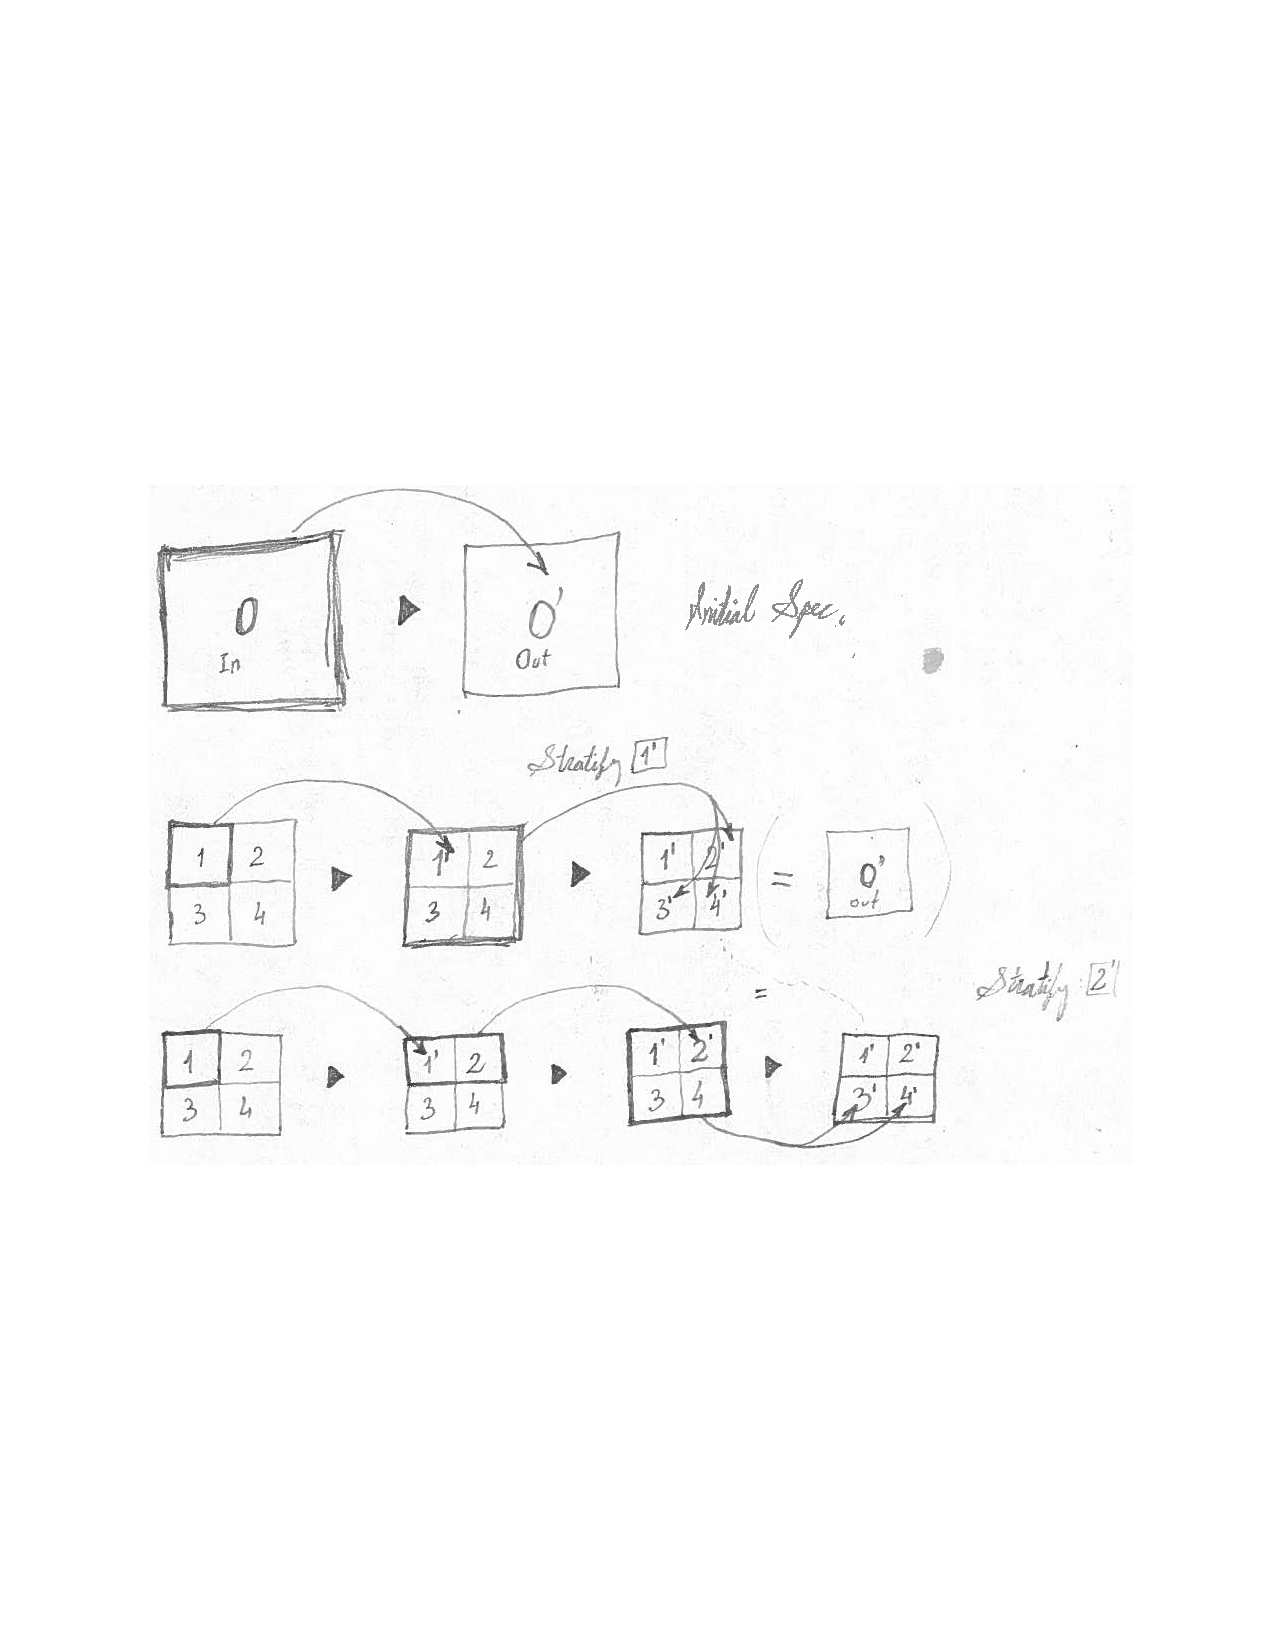
\includegraphics[width=.47\textwidth]{img/gap-stratify2}\\
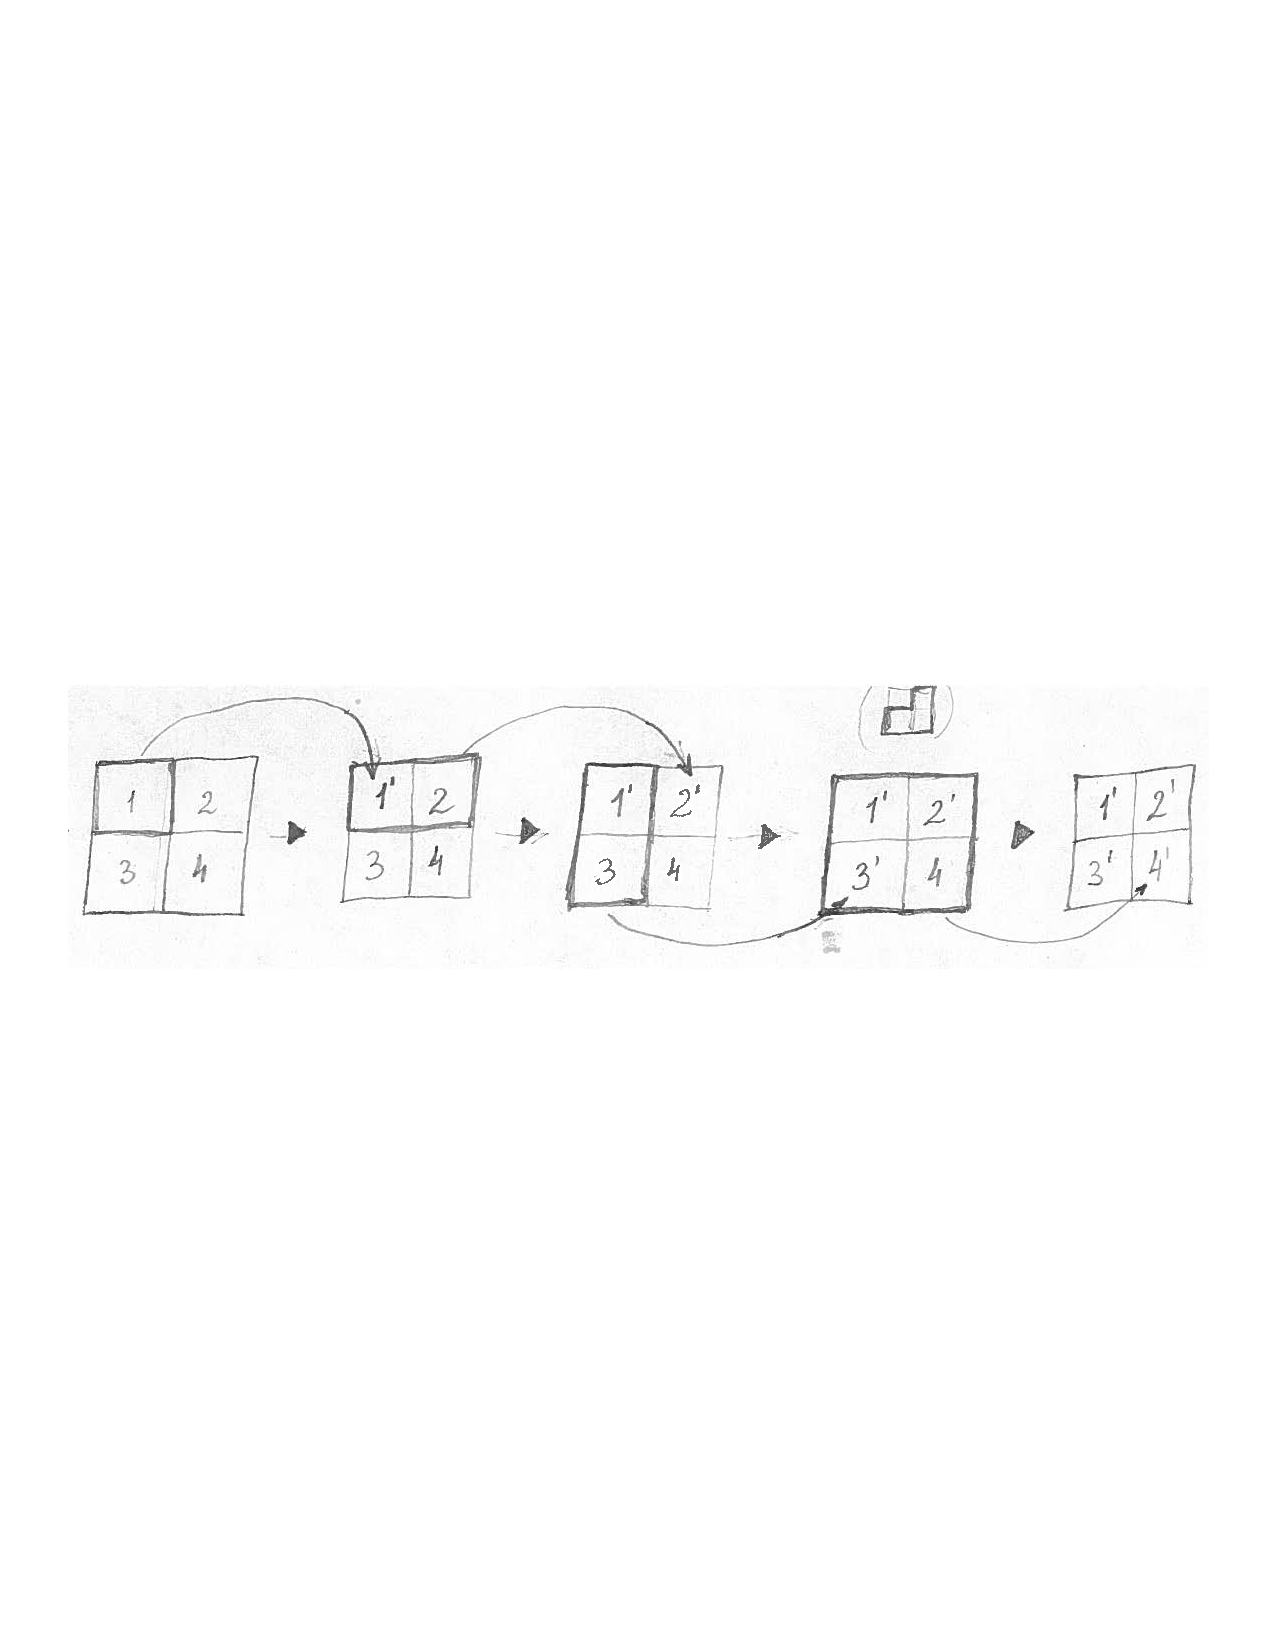
\includegraphics[width=.47\textwidth]{img/gap-stratify3}
\caption{
  Stratification steps for phase ``A'' of Simplified Gap.}
\end{figure}

\hrule
\bigskip
